\documentclass[a4paper,12pt,oneside]{article}

% Imported packages
\usepackage[english]{babel}
\usepackage[T1]{fontenc}
\usepackage[utf8]{inputenc}
\usepackage{float}
\usepackage{graphicx}
\usepackage{color}
\usepackage{amssymb}
\usepackage{amsmath}
\usepackage{bm}
\usepackage{listings}
\usepackage{comment}
\usepackage{geometry}
\usepackage{wrapfig}
\usepackage{subfigure}
\usepackage{hyperref}
\usepackage{cancel}

% Margin dimensions settings
\geometry{a4paper,top=2cm,bottom=2cm,left=2cm,right=2cm,%
	heightrounded,bindingoffset=5mm}

% x bar for UTF-8 encoding
\DeclareUnicodeCharacter{304}{$ \bar{x} $}

% Enumeration settings
\renewcommand\thesubsection{\thesection.\alph{subsection}}

% Code visualization settings
\lstset{basicstyle=\small\ttfamily}

% Code design settings
\lstset{language=Matlab}

% Included images path
\graphicspath{{Images/}}

% Document information
\title{Fundamentals of Vibration Analysis and Vibroacoustics \\
	Module 2 - Vibroacoustics of Musical Instruments \\
	Assignment 1 - Axial vibration of undamped and damped bars}
\author{Bombaci Nicola 10677942 \\
	Fantin Jacopo 10591775 \\
	Intagliata Emanuele 10544878}
\date{June 2020}


\begin{document}

\maketitle

\vspace{100pt}

\section*{System schematic and parameters}

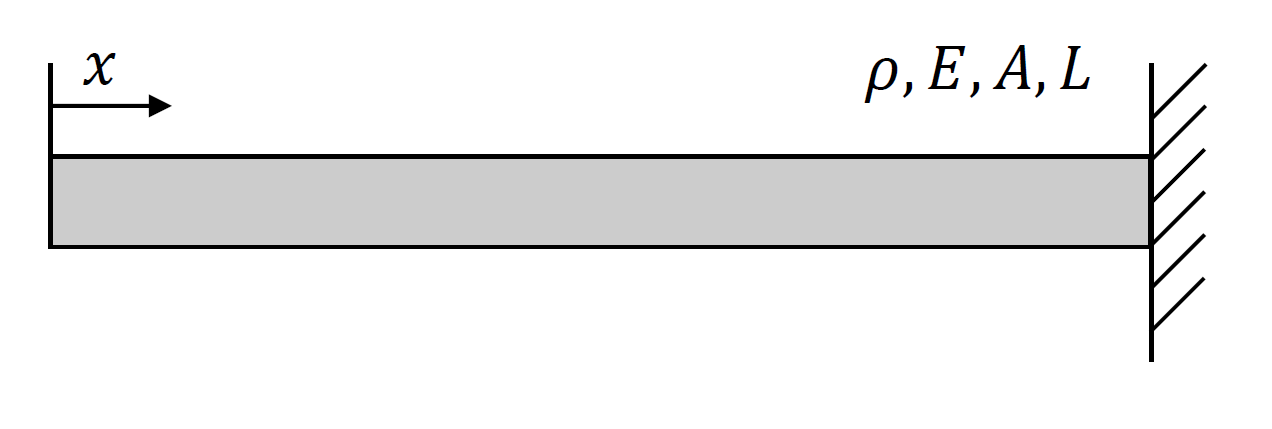
\includegraphics[width=0.9\textwidth]{system_schematic}

\vspace{30pt}

\[
	\rho = 2700 \, \text{kg/m\textsuperscript{3}} ~ \text{,} ~ E = 70 \, \text{GPa} %
		~ \text{,} ~ L = 2 \, \text{m} ~ \text{,} ~ b = h = 0.05 \, \text{m}
\]

\clearpage


\section{Natural frequencies and mode shapes \\ in free-fixed configuration}
\label{sec:nat_freqs_and_mode_shapes_free_fixed}

Starting from the one-dimensional wave equation and applying it for the axial displacement $ s(x,t) $ of point at position $ x $ at time $ t $:

\[
	\frac{\partial^2 s(x,t)}{\partial x^2} = %
		\frac{1}{c^2} \, \frac{\partial^2 s(x,t)}{\partial t^2}
\]

We already know that a solution to the equation is the standing wave expression, where space and time dependencies are separated by the mode shape function $ \Phi(x) $ and the complex exponential $ G(t) $:

\[
	s(x,t) = \Phi(x) \, G(t) = %
		\bigl(A \, \sin(kx) + B \, \cos(kx)\bigl) \, e^{j \omega \, t}
\]

\vspace{10pt}

The bar is in free-fixed condition, so the boundary conditions are

\[ \begin{cases}
	N(0,t) = E \, S \, \frac{\partial s(x,t)}{\partial x} \Big|_{x=0} = 0 %
		~ \Rightarrow ~ E \, S \, A \, k \, e^{j \omega \, t} = 0 %
		~ \Rightarrow ~ A = 0 ~ \text{($ k = 0 $ is a trivial solution)} \\
	s(L,t) = 0 ~ \Rightarrow ~ B \, \cos(kL) = 0 ~ \Rightarrow ~ %
		k^{\textup{fr-fx}^{(i)}} = \frac{2i - 1}{2L} \pi %
		~ \text{,} ~ i = 1,2,...,\infty
\end{cases} \]

where $ S $ denotes the area of the bar's cross-section and $ N $ the normal axial load. From the second condition, the natural frequencies can be directly retrieved:

\[
	f_\textup{n}^{\textup{fr-fx}^{(i)}} = %
		\frac{\omega_\textup{n}^{\textup{fr-fx}^{(i)}}}{2 \pi} = %
		\frac{c \, k^{\textup{fr-fx}^{(i)}}}{2 \pi} = %
		\frac{2i - 1}{4L} \sqrt{\frac{E}{\rho}} ~ \text{,} ~ i = 1,2,...,\infty
\]

Our analysis is restricted to the frequency band $ [0, f_\textup{max}] = [0, 10k] \, $ Hz, so $ i $ assumes values within a finite set of indices:

\[ \begin{split}
	& f_\textup{max} = \frac{2 \, i^\textup{fr-fx}_\textup{max} - 1}{4L} %
		\sqrt{\frac{E}{\rho}} \\
	& \Rightarrow ~ \lfloor i^\textup{fr-fx}_\textup{max} \rfloor = %
		\Biggl\lfloor 2 L f_\textup{max} %
		\sqrt{\frac{\rho}{E}} + \frac{1}{2} \Biggr\rfloor = \lfloor 8.35 \rfloor = 8
\end{split} \]

So $ i = 1,2,...,8 $ and the resulting natural frequencies are

\[
	\mathbf{f_n^{fr-fx}} =	\begin{bmatrix}
														636.47		& 1909.40	& 3182.30	& 4455.30 %
														& 5728.20	& 7001.20	& 8274.10	& 9547.00
													\end{bmatrix}
\]

The mode shapes $ \Phi^{\textup{fr-fx}^{(i)}}(x) $ are then, considering the constant coefficient $ B = 1 $,

\[
	\Phi^{\textup{fr-fx}^{(i)}}(x) = \cos(k^{\textup{fr-fx}^{(i)}} x) =
		\cos\biggl(\frac{2i - 1}{2L} \pi \, x\biggr) ~ \text{,} ~ i = 1,2,..,8
\]

We hereby show them plotting the longitudinal oscillation amplitude of each point of the bar versus the points position. As expected, the oscillation of the free end always has maximum amplitude.

\begin{figure}[h]
	\hspace{-70pt}
	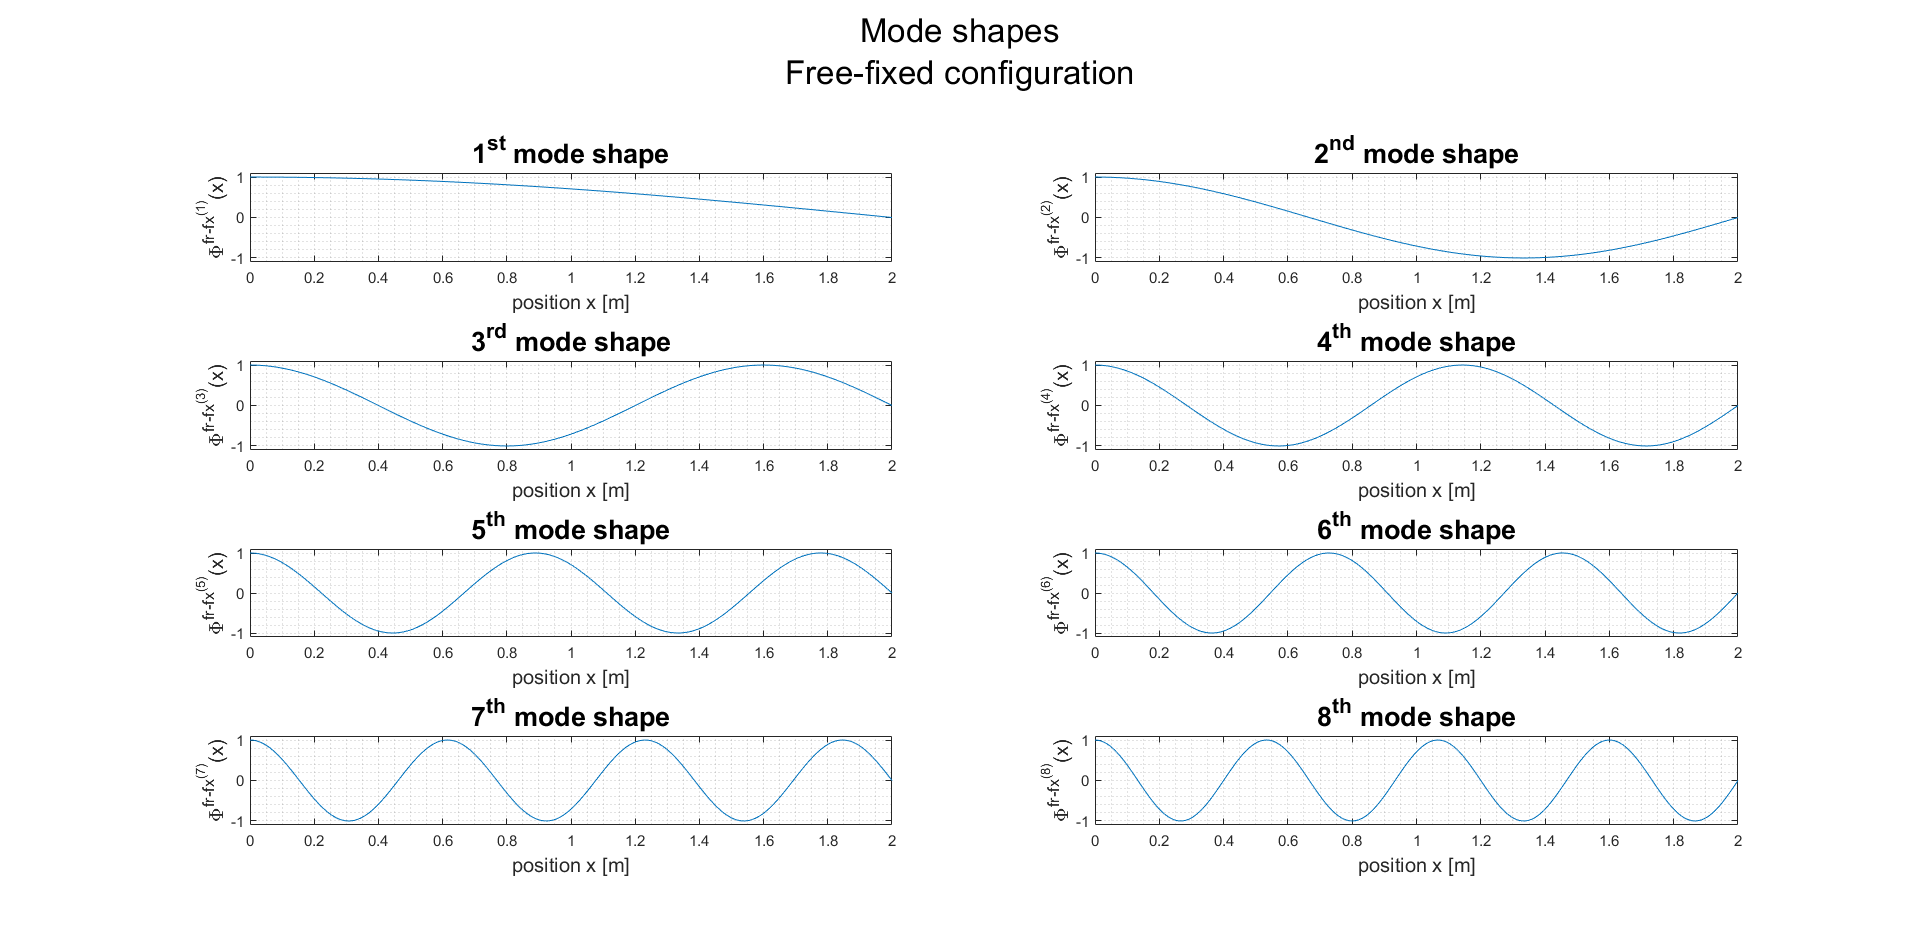
\includegraphics[scale=0.4]{mode_shapes_free_fixed}
\end{figure}


\section{Natural frequencies and mode shapes \\ in free-free configuration}

Differently, in a free-free configuration of the bar the boundary condition on the normal force $ N $ is applied to the right end of the bar too:

\[ \begin{split}
	& \begin{cases}
			N(0,t) = E \, S \, \frac{\partial s(x,t)}{\partial x} \Big|_{x=0} = 0 %
				~ \Rightarrow ~ E \, S \, A \, k \, e^{j \omega \, t} = 0 %
				~ \Rightarrow ~ A = 0 ~ \text{($ k = 0 $ is a trivial solution)} \\
			N(L,t) = E \, S \, \frac{\partial s(x,t)}{\partial x} \Big|_{x=L} = 0 %
				~ \Rightarrow ~ - E \, S \, B \, k \, \sin(kL) = 0 ~ \Rightarrow ~ \sin(kL) = 0
	\end{cases}	\\
	& \hspace{150pt}~ \Rightarrow ~ %
		k^{\textup{fr-fx}^{(i)}} = \frac{i}{L} \pi ~ \text{,} ~ i = 0,1,...,\infty
\end{split} \]

So the natural frequencies are computed from $ k^{\textup{fr-fr}^{(i)}} $ as before:

\[
	f_\textup{n}^{\textup{fr-fr}^{(i)}} = %
		\frac{\omega_\textup{n}^{\textup{fr-fr}^{(i)}}}{2 \pi} = %
		\frac{c \, k^{\textup{fr-fr}^{(i)}}}{2 \pi} = %
		\frac{i}{2L} \sqrt{\frac{E}{\rho}} ~ \text{,} ~ i = 0,1,...,\infty
\]

This time the maximum value for index $ i $ is

\[ \begin{split}
	& f_\textup{max} = \frac{i^\textup{fr-fr}_\textup{max}}{2L} %
		\sqrt{\frac{E}{\rho}} \\
	& \Rightarrow ~ \lfloor i^\textup{fr-fr}_\textup{max} \rfloor = %
		\Biggl\lfloor 2 L f_\textup{max} \sqrt{\frac{\rho}{E}} \Biggr\rfloor = %
		\lfloor 7.86 \rfloor = 7
\end{split} \]

So $ i = 0,1,...,7 $ and the corresponding natural frequencies are

\[
	\mathbf{f_n^{fr-fr}} =	\begin{bmatrix}
																	0					& 1272.9	& 2545.9	& 3818.8 %
																	& 5091.8	& 6364.7	& 7637.6	& 8910.6
													\end{bmatrix}
\]

The number of resonances within $ f_\textup{max} $ is the same, but the most important consideration is about the fact the system has now a resonance at $ f = 0 $, which means a fixed amount of longitudinal displacement is added to the displacement of each point of the bar during the vibration. This value, constant in time, is called rigid motion. Ituitively, it makes perfect sense as the bar is in free-free configuration, and applying a constant force at one of the two ends, the whole bar will rigidly move in the direction of the force. The fixed-fixed configuration shows a zero-frequency component too, but it doesn't correspond to a rigid motion different from zero, but rather to absence of motion, therefore it's not includible among the system's resonances but it's rather a trivial solution of the equation of motion. The second consideration is that, while in the free-fixed case the resonance frequencies are odd integer multiples of the fundamental, in the free-free case these are all the integer multiples of the fundamental, both even and odd, which is twice that of the first case. In other words, naming $ f_0 = 636.47 \, \text{Hz} $ the fundamental frequency of the free-fixed configuration, in the first case the resonances are

\[
	\mathbf{f_n^{fr-fx}} =	\begin{bmatrix}
														f_0	& 3f_0	& 5f_0	& 7f_0	& 9f_0	& 11f_0	& 13f_0	& 15f_0
													\end{bmatrix}
\]

while in the second case

\[
	\mathbf{f_n^{fr-fr}} =	\begin{bmatrix}
														0	& 2f_0	& 4f_0	& 6f_0	& 8f_0	& 10f_0	& 12f_0	& 14f_0
													\end{bmatrix}
\]

Just like before, the resulting mode shapes $ \Phi^{\textup{fr-fr}^{(i)}}(x) $ are computed and plotted considering $ B = 1 $.

\[
	\Phi^{\textup{fr-fr}^{(i)}}(x) = \cos(k^{\textup{fr-fr}^{(i)}} x) = %
		\cos\biggl(\frac{i}{L} \pi \, x\biggr) ~ \text{,} ~ i = 0,1,...,7
\]

\begin{figure}[h]
	\hspace{-70pt}
	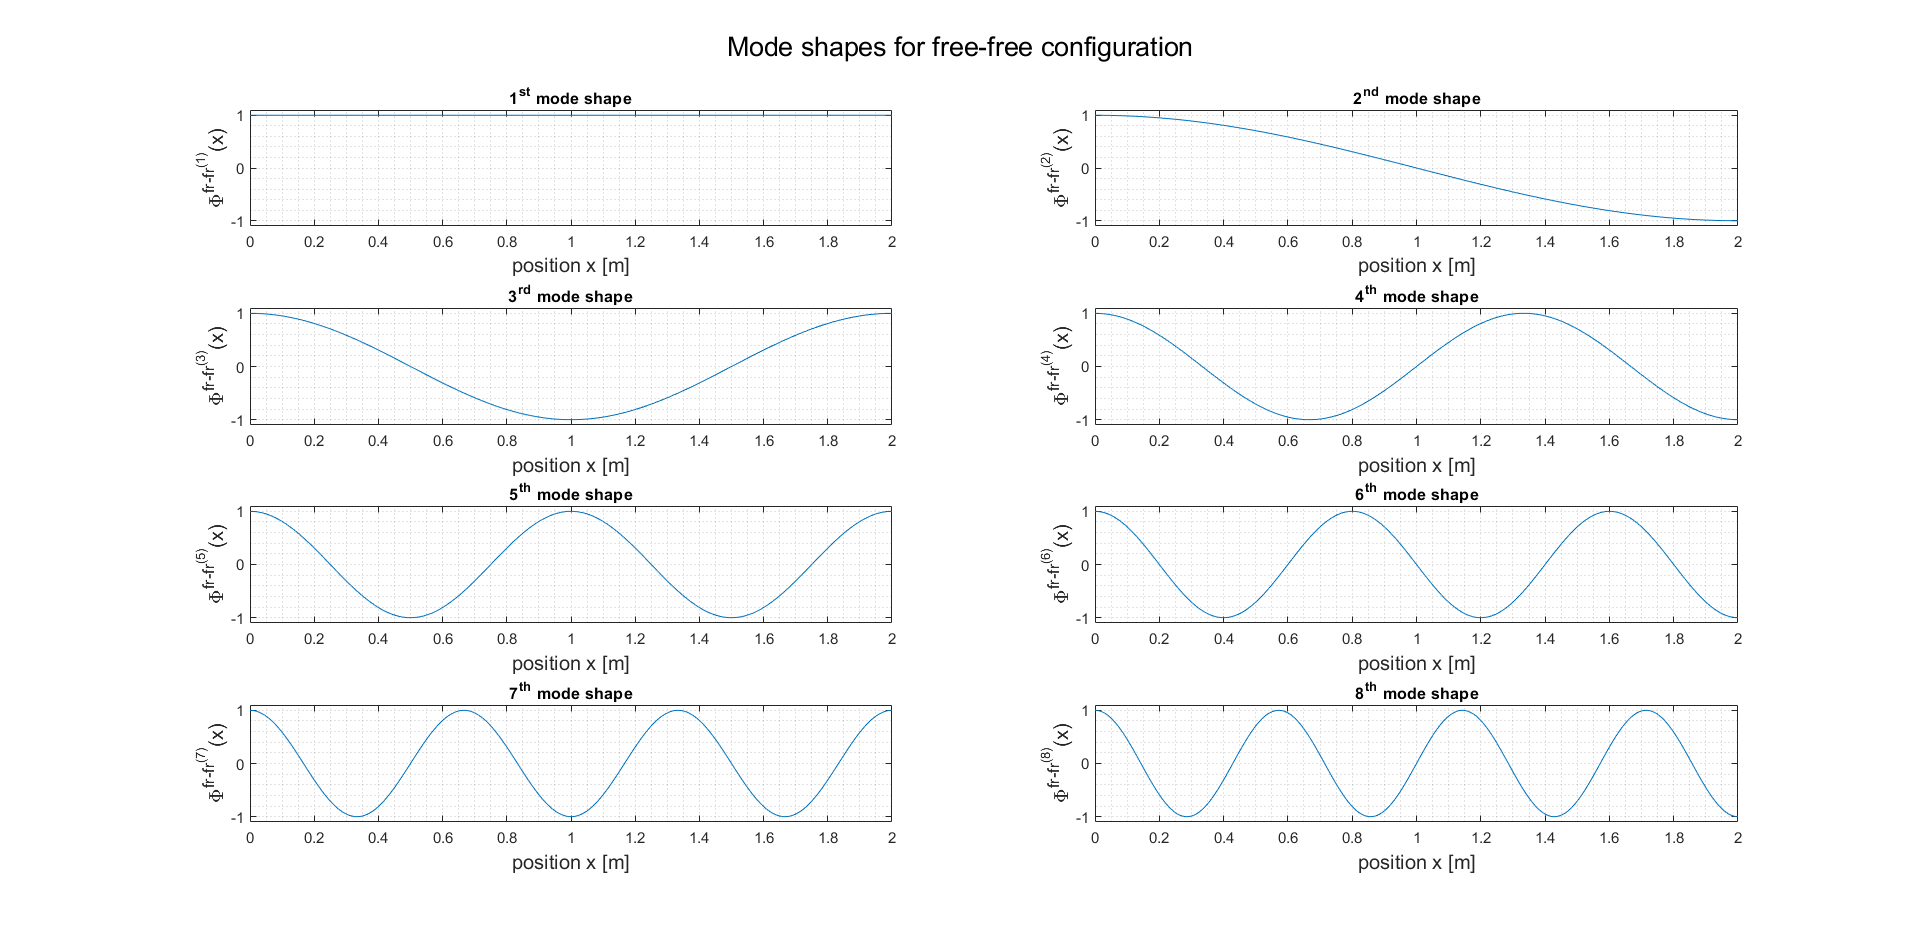
\includegraphics[scale=0.4]{mode_shapes_free_free}
\end{figure}


\section{Frequency Response Functions \\ in free-fixed configuration}
\label{sec:frfs}

For computing the system's FRFs, we're considering a harmonic force $ F(t) = F_0 \, e^{j \omega \, t} $ acting at the bar free end, so the application point is at $ \bar{x} = 0 $, while the bar points for which the FRF is computed are at $ \bar{x} = \frac{L}{2} $ and $ \bar{x} = \frac{L}{5} $. We're asked to find the FRFs in three different cases.

\subsection*{Case 1: undamped bar (standing wave solution)}

Considering the bar as not affected by energy losses during its vibration, a solution of the wave equation is seeked, resulting in non-attenuating standing waves superposition. Like we did for the natural frequencies of the bar, we find the coefficients $ A $ and $ B $ appearing in the expression for $ \Phi(x) $ imposing the same boundary conditions as in the free-fixed condition, but accounting for the external harmonic excitation too:

\[ \begin{cases}
	N(0,t) = E \, S \, \frac{\partial s(x,t)}{\partial x} \Big|_{x=0} + %
		F_0 \, e^{j \omega \, t} = 0 %
		~ \Rightarrow ~ E \, S \, A \, k \, e^{j \omega \, t} + %
		F_0 \, e^{j \omega \, t} = 0 %
		~ \Rightarrow ~ A = -\frac{F_0}{E \, S \, k} \\
	s(L,t) = 0 ~ \Rightarrow ~ -\frac{F_0}{E \, S \, k} \, \sin(kL) + B \, \cos(kL) = 0 %
		~ \Rightarrow ~ B = \frac{F_0 \, \sin(kL)}{E \, S \, k \, \cos(kL)}
\end{cases} \]

\[
	\Rightarrow s(x,t) = \bigl(A \, \sin(kx) + B \, \cos(kx)\bigl) \, e^{j \omega \, t} =
		\frac{\sin\bigl(k(L - x)\bigr)}{E \, S \, k \, \cos(kL)} \,
		F_0 \, e^{j \omega \, t}
		~ \Rightarrow ~ \frac{\sin\bigl(k(L - x)\bigr)}{E \, S \, k \, \cos(kL)} \, F(t)
\]

from which the FRF can be retrieved, considering the frequency dependency in place of the time dependency:

\[
	H^{SWS}(\omega) = \frac{s(x, \omega)}{F(\omega)} = %
		\frac{\sin\bigl(k(L - x)\bigr)}{E \, S \, k \, \cos(kL)}
\]

\vspace{20pt}

The FRF connecting the specific point $ \bar{x} $ on the x-axis to the force applied at the free end is then:

\begin{equation}
\label{eqn:frf_sws}
	H^{SWS}_{\bar{x}}(\omega) = H^{SWS}(\omega)\big|_{x = \bar{x}} = %
		\frac{\sin\bigl(k(L - \bar{x})\bigr)}{E \, S \, k \, \cos(kL)}
\end{equation}

\vspace{20pt}

We hereby show the amplitude and phase plots for both the points we want to compute the response of. Note that, for $ \bar{x} = \frac{L}{5} $, two resonances are missing, precisely those of mode 3 and 8, indicating that these modes are non-observable modes in point $ \bar{x} = \frac{L}{5} $. This comes in accordance with the mode shapes we found in section \ref{sec:nat_freqs_and_mode_shapes_free_fixed}: the point $ \bar{x} = \frac{L}{5} = 0.4 \, \text{m} $ is indeed a node for mode shapes 3 and 8, while $ \bar{x} = \frac{L}{2} $ is a node for no mode, due to the asymmetric boundary conditions we imposed, due to asymmetric bar configuration in turn.

\clearpage

\begin{figure}[h]
	\vspace{50pt}
	\centering
	\def\svgwidth{\columnwidth}
	\input{images/frfs_standing_wave_solution.pdf_tex}
\end{figure}

\subsection*{Case 2: damped bar (wave propagation solution)}

In this second case, the bar is damped, so the energy loss factor $ \eta $ is introduced. This represents the viscoelasticity of the bar, which is now not purely elastic as in an undamped one, and is comprised in a new, complex, Young's modulus, which leads to a new wave equation:

\[ \begin{split}
	& E' = E \, (1 + j \eta) ~ \Rightarrow ~
		E' \,	\frac{\partial^2 s(x,t)}{\partial x^2} =
		\rho \, \frac{\partial^2 s(x,t)}{\partial t^2} \\
	& ~ \Rightarrow ~ c' = \sqrt{\frac{E'}{\rho}} = \sqrt{\frac{E \,(1 + j \eta)}{\rho}}
		= c \, \sqrt{1 + j \eta} \approx
		c \, \sqrt{\frac{1 + \frac{\eta^2}{4}}{1 + \frac{\eta^4}{16} + \frac{\eta^2}{2}} +
		j \frac{\eta}{1 + \frac{\eta^4}{16} + \frac{\eta^2}{2}}}
		= \frac{c}{1 - j \frac{\eta}{2}}
\end{split} \]

where the approximation is valid for low loss factors, e.g. order of magnitude of $ 10^{-2} $, which is our case. So the wavenumber is now

\[
	k' = \frac{\omega}{c'} = \frac{\omega}{c} \, (1 - j \frac{\eta}{2})
		= k \, (1 - j \frac{\eta}{2})
\]

Applying the new value for Young's modulus and the wavenumber to the same FRF of the previous case \eqref{eqn:frf_sws}, thus using the same boundary conditions as before, the new frequency response function is retrieved:

\[
	H^{WPS}_{\bar{x}}(\omega) = H^{WPS}(\omega)\big|_{x = \bar{x}} = %
		\frac{\sin\bigl(k'(L - \bar{x})\bigr)}{E' \, S \, k' \, \cos(k'L)}
\]

\vspace{10pt}

The corresponding magnitude and phase plots are depicted in the following figure. As we can see, the resonances are at the same frequencies as before, but the amplitude plot shows attenuated values due to the introduction of $ \eta $, and the phase plot shows not perfectly vertical jumps now.

\begin{figure}[h]
	\vspace{50pt}
	\centering
	\def\svgwidth{\columnwidth}
	\input{images/frfs_wave_propagation_solution.pdf_tex}
\end{figure}

\subsection*{Case 3: damped bar (modal superposition approach)}

Following a modal approach, we started from the theoretical result that allows us to find the bar point $ x_\textup{out} $'s steady-state oscillation amplitude as response to input external force $ F(\omega) $ applied in point $ x_\textup{in} $

\[ \begin{split}
	s(x_\textup{out}, \omega) & = %
		\sum_{i=1}^N \Phi^{(i)}(x)\big|_{x_\textup{out}} \, q_{0_i} \\
	& = \sum_{i=1}^N \frac{\Phi^{(i)}(x)\big|_{x_\textup{out}} \, %
		\Phi^{(i)}(x)\big|_{x_\textup{in}} \, F_0} %
		{-\omega^2 \, m^{(i)} + (1 + j \eta) \, k^{(i)}}
\end{split} \]

In our case:

\[ \begin{split}
	s(\bar{x},\omega) =
		\sum_{i=1}^N \frac{\Phi^{\textup{fr-fx}^{(i)}}(x)\big|_{\bar{x}} \,
		\Phi^{\textup{fr-fx}^{(i)}}(x)\big|_0 \, F_0}
		{-\omega^2 \, m^{(i)} + (1 + j \eta) \, k^{(i)}}
\end{split} \]

Dividing both sides by $ F_0 $ the expression for the FRF is derived:

\[ \begin{split}
	H^\textup{MSA}_{\bar{x}} & =
		\sum_{i=1}^N \frac{\Phi^{\textup{fr-fx}^{(i)}}(x)\big|_{\bar{x}} \,
		\Phi^{\textup{fr-fx}^{(i)}}(x)\big|_0}
		{-\omega^2 \, m^{(i)} + (1 + j \eta) \, k^{(i)}} =
		\sum_{i=1}^N \frac{\cos(k^{\textup{fr-fx}^{(i)}} x)\big|_{\bar{x}} \,
		\cos(k^{\textup{fr-fx}^{(i)}} x)\big|_0}
		{-\omega^2 \, m^{(i)} + (1 + j \eta) \, k^{(i)}} = \\
	& = \sum_{i=1}^N \frac{\cos(k^{\textup{fr-fx}^{(i)}} \bar{x})}
		{-\omega^2 \, m^{(i)} + (1 + j \eta) \, k^{(i)}}
\end{split} \]

\clearpage

The modal mass and stiffness $ m^{(i)} $ and $ k^{(i)} $ are the i-th element in the diagonal of the modal mass matrix and modal stiffness matrix respectively, and they have been retrieved as

\[ \begin{split}
	& m^{(i)} = \int_0^L \mu \, \cos^2(k^{\textup{fr-fx}^{(i)}} x) \, dx =
		\mu \, \frac{L}{2} + \frac{\sin(2 L k^{\textup{fr-fx}^{(i)}})}
		{4 \, k^{\textup{fr-fx}^{(i)}}} \\
	& k^{(i)} = \int_0^L E \, S \, \Bigl(k^{\textup{fr-fx}^{(i)}}\Bigr)^2 \,
		\sin^2(k^{\textup{fr-fx}^{(i)}} x) \, dx =
		E \, S \, \frac{L}{2} \, \Bigl(k^{\textup{fr-fx}^{(i)}}\Bigr)^2 -
		\frac{\sin(2 L k^{\textup{fr-fx}^{(i)}})}{4 \, k^{\textup{fr-fx}^{(i)}}}
\end{split} \]

\vspace{20pt}

In the following plots we're showing the resulting FRFs and a comparison between those obtained through wave propagation solution and through modal superposition approach. The FRFs obtained using the two methods coincide very thoroughly in case of $ \bar{x} = \frac{L}{2} $, beginning to diverge only at the very right end due to quasi-static contributions of modes higher than the 8\textsuperscript{th} not taken into account for the modal approach, and generally thoroughly for $ \bar{x} = \frac{L}{5} $, for which the difference between the two approaches shows up earlier than for $ \bar{x} = \frac{L}{2} $. The reason for this must be the absence of two resonance peaks, that penalizes the modal approach more than in the other case. %Taking two more modes into consideration, thus "recovering" those two missing ones, would lead to a result as precise as the one for $ \bar{x} = \frac{L}{2} $.

\vspace{150pt}

\begin{figure}[h]
	\centering
	\def\svgwidth{\columnwidth}
	\input{images/frfs_modal_superposition_approach.pdf_tex}
\end{figure}

\clearpage

\begin{figure}[h]
	\vspace{50pt}
	\centering
	\def\svgwidth{\columnwidth}
	\input{images/frfs_wps_vs_msa.pdf_tex}
\end{figure}


%parte ema
\section{Driving-point impedance \\ in free-fixed configuration}

Finally, the impedance computed at the force application point, i.e. $ \bar{x} = 0 $, is requested. 

The driving-point impedance in $\bar{x}$ is defined as:

\[
Z( \omega ) =
\frac{F(t)}{v(\bar{x},t)} =
\frac{F_0 e^{j \omega \, t}}{ 
	\frac{\partial s}{\partial t} (x,t) \vert_{\bar{x}}} =
\frac{F_0}{v_0}
\qquad with \, \bar{x} = 0.
\]

Two case studies are considered. In both cases we will consider a loss factor of $\eta = 0.01$ .

\subsection*{Case 1: damped bar (wave propagation solution)}

From the considerations we did in Section \ref{sec:frfs} (Case 2), we can write the axial displacement for a damped bar as:
\[
s(x,t) = 
		\frac{\sin\bigl(k'(L - x)\bigr)}{E' \, S \, k' \, \cos(k'L)} \,
		F_0 \, e^{j \omega \, t} 
%= \frac{ e^{j k' (L-x) t}  - e^{-j k' (L-x) t}
%}{j E' \, S \, k' \, (e^{j k' L t}  + e^{-j k' L t})} \,
%		F_0 \, e^{j \omega \, t} 		
\]
In this case we start from the wave propagation solution.


In this case the axial velocity in $\bar{x}$ is:

\[
v(\bar{x},t) = \frac{\partial s}{\partial t} (x,t) \vert_{\bar{x}} =
j \omega \frac{\sin\bigl(k'(L - \bar{x})\bigr)}{E' \, S \, k' \, \cos(k'L)} \,
		F_0 \, e^{j \omega \, t} = 
j \omega s(\bar{x},t)
\]

We can easily find that the driving-point impedance in $\bar{x} = 0$ is :


\begin{gather*}
Z_{WPS} (\omega ) =
	\frac{\cancel{F_0 e^{j \omega \, t}}}{
	j \omega \frac{\sin\bigl(k'L\bigr)}{E' \, S \, k' \, \cos(k'L)} 			\, \cancel{F_0 \, e^{j \omega \, t}}} =	
-j \frac{k'E'S \cos\bigl(k'L\bigr)}{\omega  \sin(k'L)} = \\ 
= -j \frac{
\sqrt{\frac{\rho}{E}} (1 - j \frac{\eta}{2}) E' S 
\cos\bigl(\sqrt{\frac{\rho}{E}} (1 - j \frac{\eta}{2}) L \, \omega \bigr)}
{\sin\bigl(\sqrt{\frac{\rho}{E}} (1 - j \frac{\eta}{2}) L \, \omega \bigr)}
\end{gather*} 

This last expression is the one used in our \textsc{Matlab} code to plot the driving-point impedance in the case of a damped bar, calculated starting from the wave propagation solution.

\begin{figure}[h]
	\hspace{-70pt}
	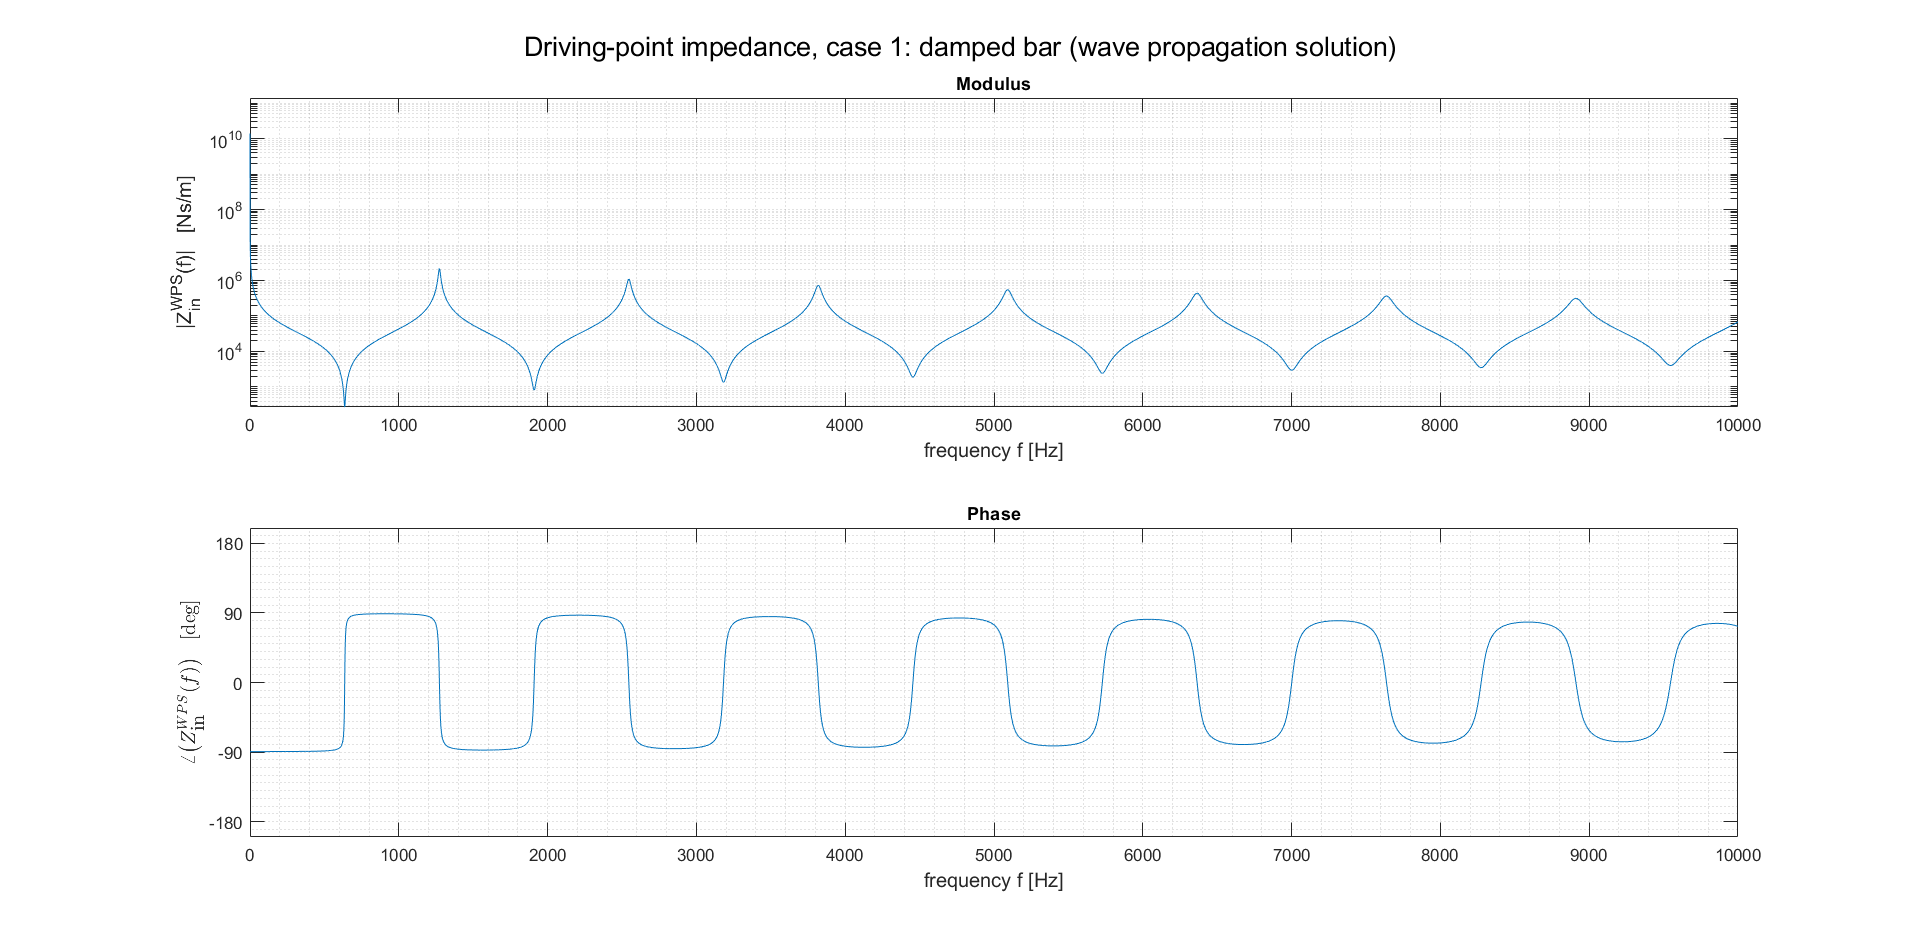
\includegraphics[scale=0.4]{impedance_wave_propagation_solution}
\end{figure}

We can briefly comment the previous plot. Being the system damped, the driving-point impedance is complex. Therefore it does not go to zero at resonance and it does not to infinite at anti resonance.
Remembering that $Z(\omega) = Z_R +jZ_I = |Z|e^{j\phi}$, the average power input introduced into or removed from the system is different from zero. It is:

\[
\overline{W} = \frac{1}{2} Z_R |v|^2 
\]

$\overline{W}$ is maximum in correspondence of the resonances, where $Z_R$ is maximum (as we can deduct from the phase plot).

\subsection*{Case 2: damped bar (modal superposition approach)}

From the considerations we did in Section \ref{sec:frfs} (Case 3), we can write the axial displacement for a damped bar as:

\[ \begin{split}
	s(\bar{x}, t) = 
		F_0 e^{j \omega \, t}
		\sum_{i=1}^N \frac{\Phi^{\textup{fr-fx}^{(i)}}(x)\big|_{\bar{x}} \,
		\Phi^{\textup{fr-fx}^{(i)}}(x)\big|_0 }
		{-\omega^2 \, m^{(i)} + (1 + j \eta) \, k^{(i)}}
\end{split} \]

In this case we start from the modal superposition approach. In this case the axial velocity in $\bar{x}$ is:

\[
v(\bar{x},t) = \frac{\partial s}{\partial t} (x,t) \vert_{\bar{x}} =
j \omega  
F_0 e^{j \omega \, t}
		\sum_{i=1}^N \frac{\Phi^{\textup{fr-fx}^{(i)}}(x)\big|_{\bar{x}} \,
		\Phi^{\textup{fr-fx}^{(i)}}(x)\big|_0 }
		{-\omega^2 \, m^{(i)} + (1 + j \eta) \, k^{(i)}} = 
j \omega s(\bar{x},t)
\]

The driving-point impedance is computed at the excitation point. Therefore $\Phi^{\textup{fr-fx}^{(i)}}(x)\big|_{\bar{x} = 0}  = 
		\Phi^{\textup{fr-fx}^{(i)}}(x)\big|_0 = 1$ .
We can easily find that the driving-point impedance in $\bar{x} = 0$ is :


\begin{gather*}
Z_{MSA} (\omega ) =
	\frac{\cancel{F_0 e^{j \omega \, t}}}{
	j \omega \cancel{F_0 e^{j \omega \, t}}
		\sum_{i=1}^N \frac{\Phi^{\textup{fr-fx}^{(i)}}(x)\big|_{\bar{x}} \,
		\Phi^{\textup{fr-fx}^{(i)}}(x)\big|_0 }
		{-\omega^2 \, m^{(i)} + (1 + j \eta) \, k^{(i)}}
	}	
= \\
= -j \frac{1}{\omega
		\sum_{i=1}^N \frac{1}
		{-\omega^2 \, m^{(i)} + (1 + j \eta) \, k^{(i)}}}
\end{gather*} 

Themodal parameters $m^{(i)}, \, k^{(i)}$ are the one calculated in Section \ref{sec:frfs} (Case 3).

This last expression is the one used in our \textsc{Matlab} code to plot the driving-point impedance in the case of a damped bar, calculated starting from the modal superposition approach. In this case $N=8$ modes are used.

\begin{figure}[h]
	\hspace{-70pt}
	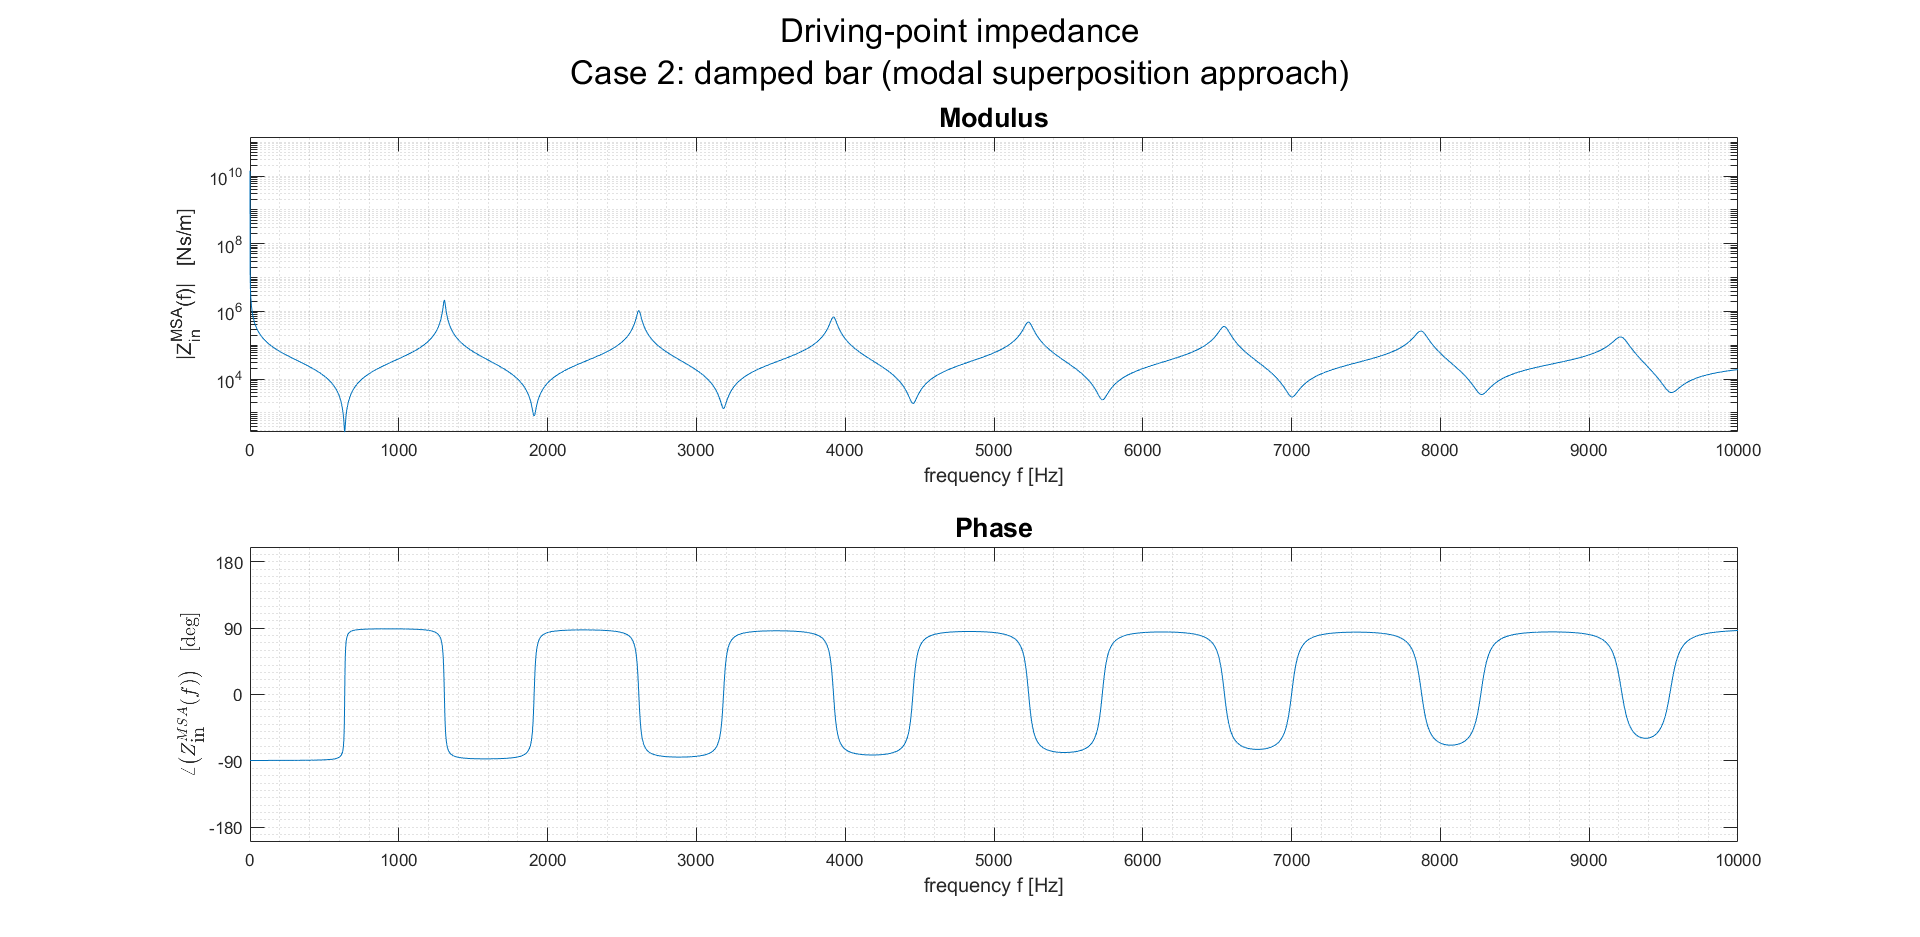
\includegraphics[scale=0.4]{impedance_modal_superposition_approach}
\end{figure}

Regarding this plot, we can derive the same conclusions we did in Case 1.
It's interesting to see how the plot changes considering only $N=5$ modes. With $N=5 modes$ only 5 resonances are considered in the model.

\begin{figure}[h]
	\hspace{-70pt}
	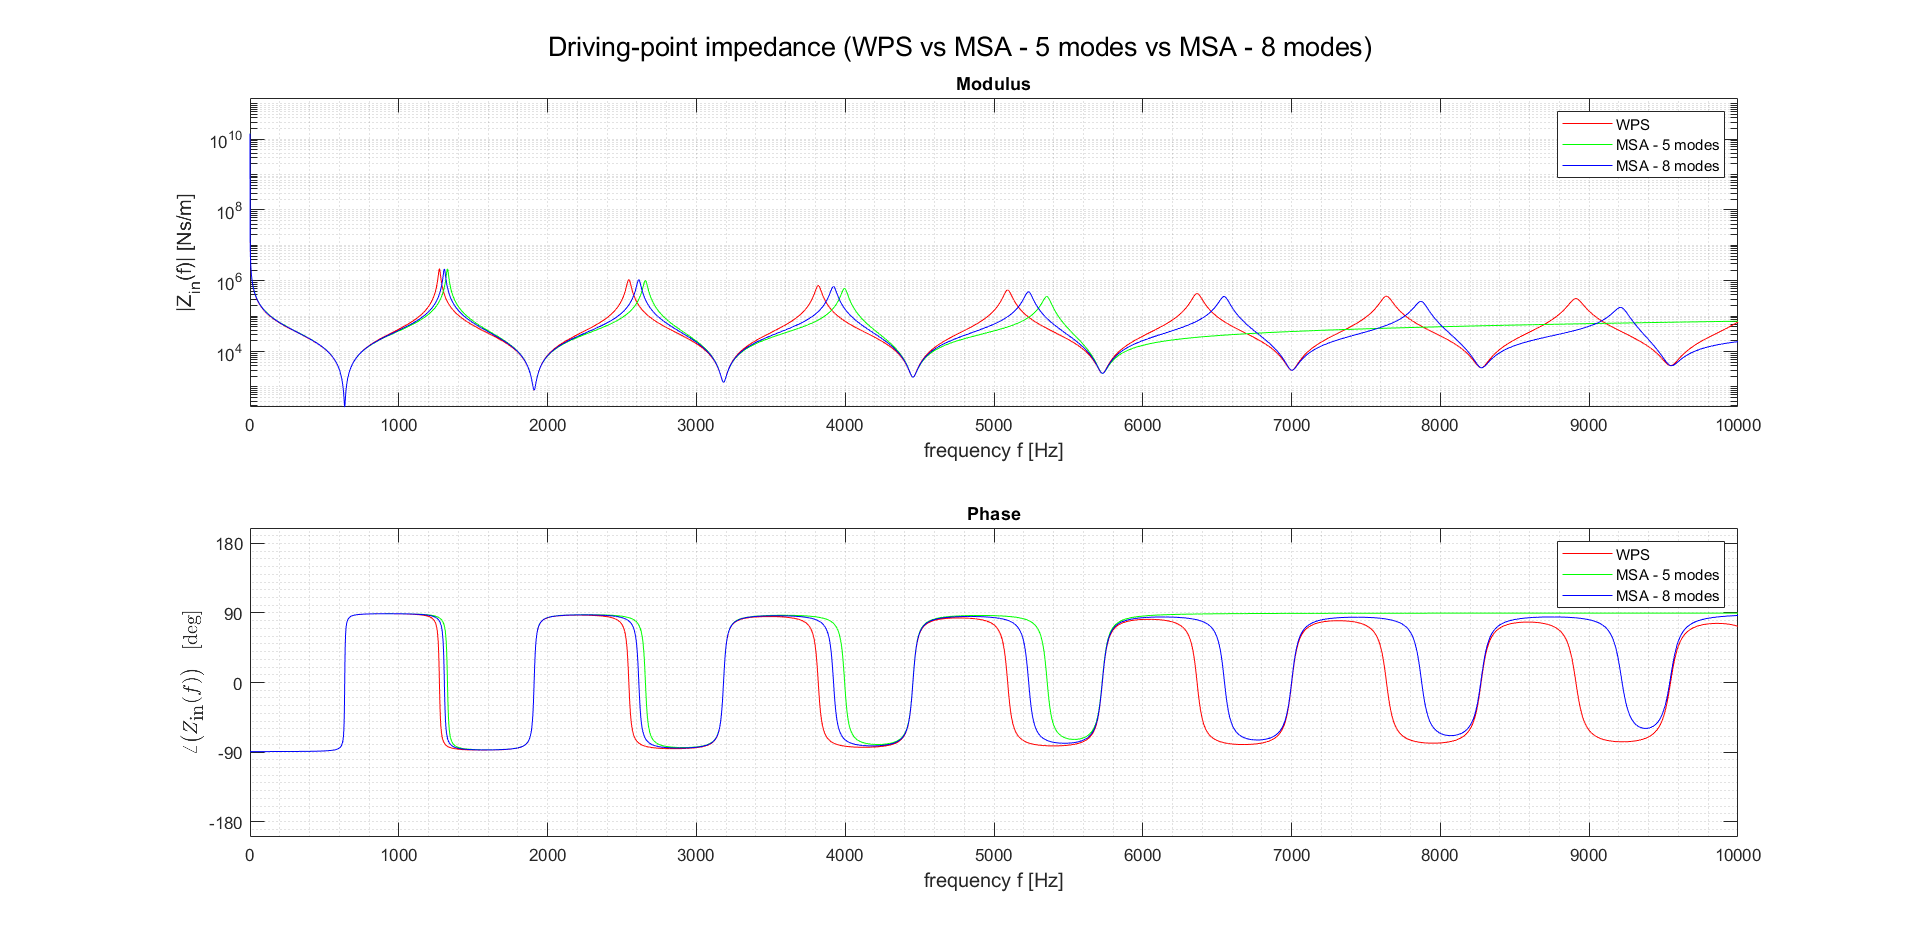
\includegraphics[scale=0.4]{impedance_wps_vs_msa}
\end{figure}

In this figure is plot the driving-point impedance found:
\begin{itemize}
\item in Case 1, starting from the wave propagation solution;
\item in Case 2, using the modal superposition approach and considering $N=8$ modes;
\item in Case 2, using the modal superposition approach and considering $N=5$ modes.
\end{itemize}

For lightly damped systems at resonance, the resonant mode is dominating the
system response. Therefore the approximation is very good.
On the contrary, at anti-resonance the approximation is worse.
That's because in anti-resonance the system response is dominating. All the modes contribute to the system response: dealing with a finite number of modes the approximation of the response is worse. Theoretically, if we had $N= \infty$ modes the solution would be exactly the same. It can be noticed that the approximation gets better if we increase the number of modes.
The higher the number of considered modes:
\begin{itemize}
\item the larger the frequency range where the driving-point impedance is accurately approximated;
\item the better the driving-point impedance is approximated in between two adjacent anti-resonance minima.
\end{itemize}

The lower the number of considered modes, the more the anti-resonance frequency tends to be overestimated.

\end{document}